% This is the aspauthor.tex LaTeX file
% Copyright 2010, Astronomical Society of the Pacific Conference Series

\documentclass[11pt,twoside]{article}
\usepackage{asp2010}

\usepackage{color}
\usepackage{amsfonts}

\usepackage{graphicx}


\resetcounters

\bibliographystyle{asp2010}

\markboth{Richard J. Baxter, Patrick Marais, and Michelle M. Kuttel}{GPU-based Acceleration of PSV Calculations}

\begin{document}
 %

\newcommand\vecc[1]{\vec{#1}}

\title{GPU-based Acceleration of Radio Interferometry Point Source
Visibility Calculations in the MEQtrees Framework} 

\author{Richard~J.~Baxter, Patrick~Marais, and Michelle~M.~Kuttel
\affil{Computer Science Department, University of Cape Town, South Africa}}

\begin{abstract}
  
Modern radio interferometer arrays are powerful tools for obtaining high
resolution, low frequency images of objects in deep space. An inverse Fourier
transform of a model sky-intensity map will produce the corresponding
\emph{Point Source Visibilities}:  the raw output of an interferometer.
Simulated visibilities can be used to test models of factors affecting the
accuracy of observed data, such as radio frequency interference. We describe a
GPU/CUDA implementation of the Point Source Visibility calculation module
within the MeqTrees software suite.  For a large numbers of sources, we
achieve an $18\times$ speed-up over the existing CPU module, with the parallel
component running up to $120\times$ faster. With modifications to the MeqTrees
memory management system to incorporate GPU memory operations, a speed-up of
$24\times$ is achievable.

\end{abstract}


\section{Introduction}

Radio Interferometry employs multiple radio receiving elements  to enhance the
resolution and sensitivity of astronomical observations. While single dish
telescopes convert the electromagnetic radiation directly into an image of the
sky (or \emph{sky-intensity map}), interferometers calculate interference
patterns between pairs of receiving elements to produce points on the
Fourier/UV plane (termed \emph{visibilities}).  A subsequent Fourier transform
operation produces the image plane, or \emph{sky map}. This transformation
usually discretises the Fourier samples (the visibilities) onto a uniform grid
and then computes the synthesised image with a Fast Fourier Transform.  This
is far less computationally intensive than a direct Fourier transform on a
per-visibility basis, but introduces slight image artefacts.  The reverse
process --- conversion from a sky-map comprising a collection of point sources
to the corresponding Fourier-plane point source visibilities  with an inverse
Fourier transform --- is used in the testing of Radio Frequency Interference
(RFI) models.  These simulated point source visibilities (PSVs) are defined by
the interferometer layout, frequency bands, time intervals, and a point-source
model of the sky.


\emph{MeqTrees} is a software package used for both third-generation
calibration (3GC) of radio interferometers and for  visibility simulation.
MeqTrees currently contains a node for PSV simulation which is very
computationally expensive and has potential for parallel acceleration with
commodity Graphics Processing Units (GPUs). \label{sec:cuda}  Modern GPUs were
developed for computer gaming to render 3D scenes at high frame rates. With
the development of general application programming interfaces for GPUs, such
as nVidia's \emph{Compute Unified Device Architecture} (CUDA), these low-cost,
highly parallel accelerators are increasingly used for more general-purpose
computing. In this work, we accelerate the direct Fourier transform visibility
calculations performed by PSV component of the \emph{MeqTrees} framework using
CUDA to export the module to a GPU.  Despite the introduction of additional
overheads, such as copying of data to and from the GPU device,  we achieve
good performance, especially with CUDA-specific optimisations such as memory
coalescing and  use of shared memory.


\section{Methods}
\subsection{Calculation of Point Source Visibilites}
\label{sec:meqtrees}

Unlike single dish telescopes, interferometers do not have a simple
relationship between signal and data: a \emph{Measurement Equation}
(incorporating correlation, Fourier transform, phase shifts, and factors such
as radio frequency interference) transforms the received signal into useful
data.  The \emph{Radio Interferometry Measurement Equation} (RIME)
reformulates the classic radio interferometry visibility equation into a more
robust and general equation based on \emph{Jones matricies}
\citep{Smirnov2011}. RIME calculates the signal $V_{pq}$ that two
interferometer antennae, $p$ and $q$, will measure over period of time ($t_0,
t_1$)  and  frequency range $(\nu_0, \nu_1)$, given a number of simulated
sources, $\vecc{S}$, as:

\begin{equation}
V_{pq} = \sum_s^{\vecc{S}}
\mbox{sinc}\frac{\Delta\Psi}{2}\mbox{sinc}\frac{\Delta\Phi}{2}
B\exp\left({-2\pi i\frac{\nu}{c}(\vecc{u}_{tpq}\vecc\sigma_s)}\right)
\label{eq:RIME}
\end{equation}
where
$\Delta\Psi = \mbox{arg }V_{pq}(t_1,\nu_m) - \mbox{arg
}V_{pq}(t_0,\nu_m), 
\Delta\Phi = \mbox{arg }V_{pq}(t_m,\nu_1) - \mbox{arg
}V_{pq}(t_m,\nu_0),$
$\mbox{and } t_m = (t_0 + t_1)/2, \nu_m = (\nu_0 + \nu_1)/2 $

Here $\mbox{arg}$ denotes the complex argument or complex angle,
$\vecc{u}_{tpq}$ is the relative distance between $p$ and $q$ at time $t$,
$B_s$ is the polarised cross-correlated intensity of source $s$ and
$\vecc\sigma_s$ is the spherical location of source $s$. $\Delta\Psi$ and
$\Delta\Phi$ are smearing factors accounting for measurements over a
\emph{range} of time and frequency rather than at a single point and single
frequency value.\citep{Smirnov2011, Taylor1999}. Our principle
aim is to accelerate the MeqTrees implementation of this equation.



\subsection{CUDA and GPUs}

A CUDA GPU contains a number of Streaming Multiprocessors (SMs), each
comprising up to 48 scalar processors, or \emph{cores}.   CUDA has a C-like
syntax that is interoperable with standard C and C++. CUDA code is written in
functions called \emph{kernels}.  Kernels are compiled and then deployed to a
CUDA-capable device, where they are executed in parallel over thousands of
threads running on the GPU's many cores.   Threads are grouped into blocks and
execution of each block is independent, with no guarantee of block execution
order and no direct mechanism for inter-block communication. Threads within
the same block can communicate via shared memory.  The layout of thread blocks
can greatly affect \emph{occupancy} of the SM: the ratio of the number of
active thread blocks that an SM can hold resident at any once time to the
maximum number of thread blocks that an SM can hold. Occupancy is a useful
metric for determining the computational efficiency of the SMs. A high
occupancy means many threads available  for swapping and memory latency
hiding. Whilst higher occupancy does not necessarily mean better performance,
a low occupancy usually leads to an inability to fully hide latency.

CUDA devices have access to both \emph{on-chip} and \emph{off-chip} memory.
On-chip memory is analogous to CPU register and cache memory: it is very fast
to access (1-2 clock cycles), but limited in size (100KB-1MB). Off-chip memory
(on-board DRAM) is slower to access (400-600 clock cycles) but far larger (up
to 1GB). GPUs hide global memory latency by swapping out threads
waiting for memory requests for blocks of threads ready to perform
calculations. For this, sufficient threads are required, but too
many threads result in contention for limited register- and shared memory.
Another strategy is to coalesce memory accesses:  combine a number of
simultaneous contiguous memory accesses into one request.



\subsection{Implementation} 

\label{sec:shared-memory}
\label{sec:multiple-sources-per}

We aim to accelerate Eqn \ref{eq:RIME}, which we  decompose into its three
intrinsic dimensions --- \emph{sources}, \emph{time} and \emph{frequency}
(Fig.~\ref{fig:shared_v_global}~Left). A visibility calculation is applied to
each point source, $s$, across each time-bucket, $t$, and frequency-band,
$\nu$: a SIMD paradigm well-suited to GPU implementation.  A GPU thread is
assigned to each point in the 3D data set ($t\times \nu \times s$) which is
then reduced to a 2D array ($t\times \nu$). MeqTree computes equations
described as expression ``trees'' which are made up of nodes. The PSV
calculation tree is complex,  with multiple nodes  describing
Eqn~\ref{eq:RIME}.  To reduce inter-node overheads, we simplified the
implementation to use a single computation node, or monolithic `tree', which
was ported to the GPU with CUDA. This is advantageous as only one CUDA
implementation is required for the entire equation. Separate CUDA
implementations for each individual operation would both increase development
time and degrade performance through too many kernel invocations.

We developed three CUDA kernels for our GPU implementation of the PSV
algorithm: a visibility kernel, a reduction kernel and a reorder kernel. After
the input data is copied to the GPU device, the visibility kernel calculates
the data cube of visibilities.  The reduction kernel then sums (reduces) the
data over all sources, after which the reorder kernel packs the data into
contiguous memory to be copied back to CPU RAM with one copy command. This
coalescing reorder step avoids the overhead of multiple copy commands. The
visibility kernel takes up the majority of GPU execution time, with each
thread computing multiple ($m$) sources instead of just $1$. This approach is
memory efficient: storage space for $s$ sources is reduced to space for $s/m$
sources ($1$ thread stores results for $m$ sources). To reduce the number of
slow global memory accesses, we use shared memory in the visibility kernel for
intermediate calculations, only writing to global memory once the final
accumulated value has been calculated.

We tested our CUDA PSV node by comparison with the existing MeqTrees CPU node
using an Intel i5 2.66GHz processor (only one core employed) and an nVidia
GeForce GTX470.


\section{Results and Discussion}

\begin{figure}
\begin{center}
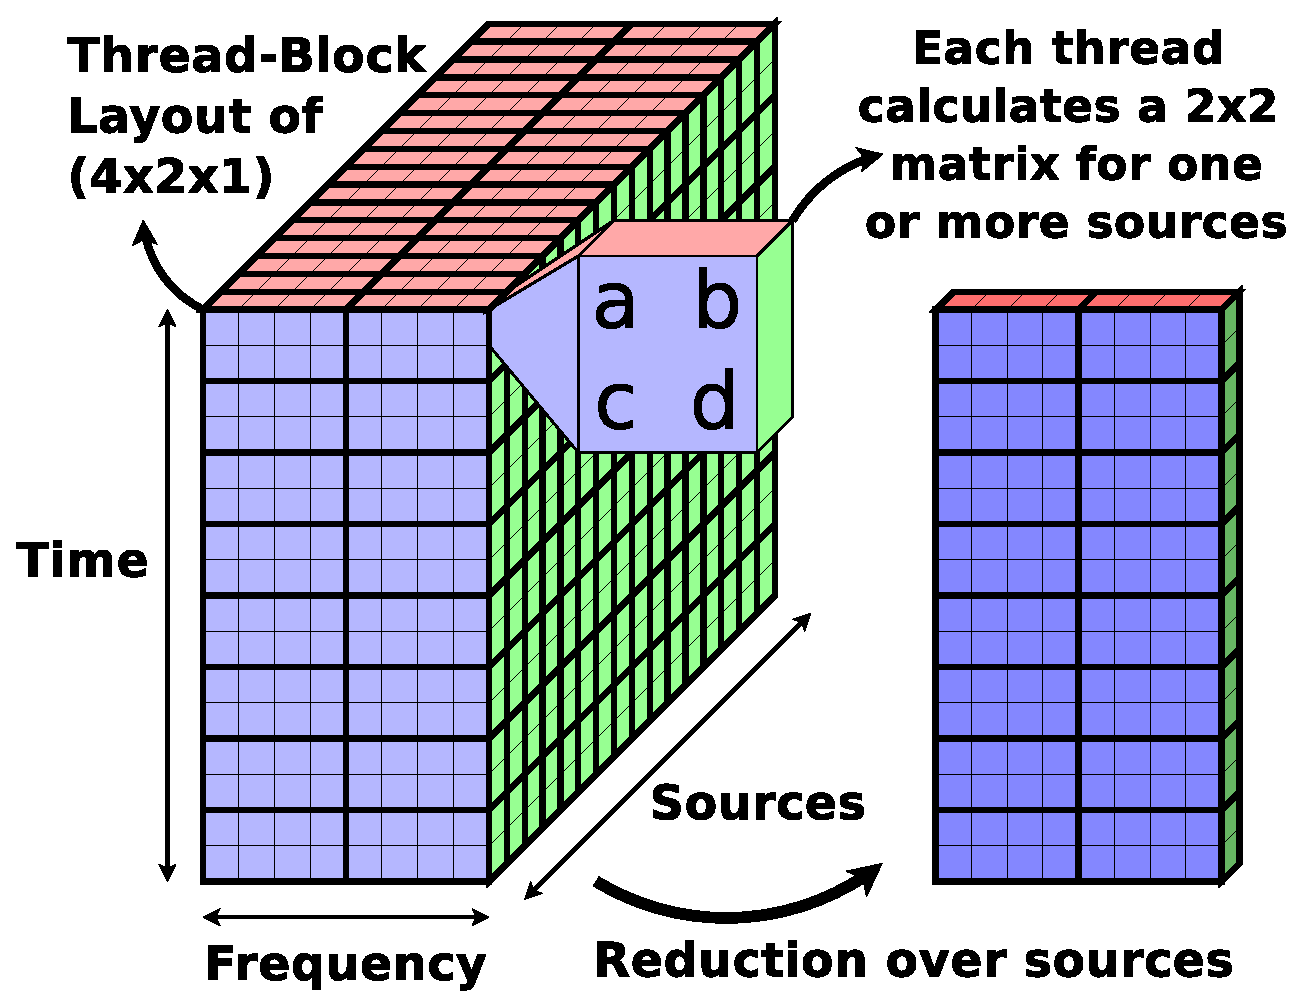
\includegraphics[scale = 0.25]{O02_f1}
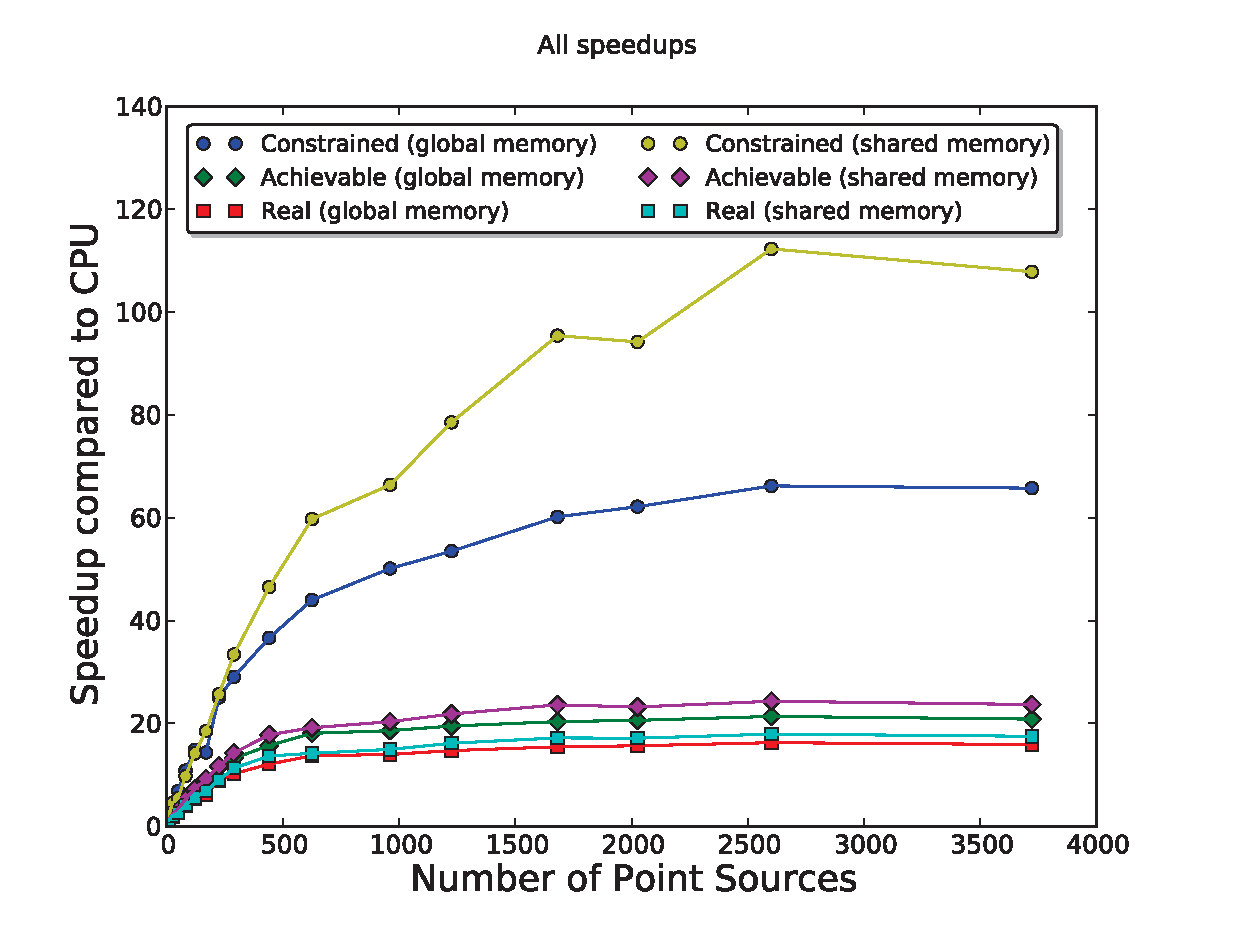
\includegraphics[scale = 0.30]{O02_f2}
\end{center}

\caption{ Left:~The data cube is reduced over the source dimension into a 2D
array. Right:~Comparison of the three speed-up metrics  ---
\emph{Real}, \emph{Achievable} and \emph{Constrained}  ---
with shared memory as compared to global memory. }

\label{fig:shared_v_global} 
\end{figure}


Our CUDA implementation shows a $18\times$ speed-up over the CPU
(Fig.~\ref{fig:shared_v_global}~Right, light~blue~line). This was achieved
through the shared memory optimisation explained above, as well as optimization
of  thread-block layouts, or \emph{occupancy}.     
MeqTrees has a ``...straightforward but very powerful scheme of
\emph{dependency tracking} [that] allows a node to figure out when a result
may be usefully cached...'' \citep{Noordam2011}. However,  the mechanisms that
allow for persistent allocation and storage are only currently implemented for
CPU memory.
This leaves all GPU node executions agnostic to any previous allocations in
any other GPU node and causes many unnecessary deallocations and re-
allocations of GPU memory. Any future MeqTrees GPU implementation will require
a persistent memory management system for GPU memory. With such a system, we
calculate (by subtraction of time taken in memory operations from the total
GPU running time) that speed up can reach $24\times$ with use of shared memory
(Fig.~\ref{fig:shared_v_global}~Right, pink~line). When just the
parallelisable parts of code are compared (without the serial overhead in
MeqTrees), we find that the GPU executes over $120\times$ faster that the CPU
(Fig.~\ref{fig:shared_v_global} Right, yellow line). Although the impact of
shared memory over global memory is small overall (between $10\%$ to $20\%$),
the the use of shared memory halves the execution time of the parallelisable
sections of code (Fig.~\ref{fig:shared_v_global} Right,
yellow~and~blue~lines). The large difference points to a potential bottleneck
in the MeqTrees framework: for the CPU version, MeqTrees overhead accounts for
an acceptable $4\%$ of the total running time. However, with the faster
running time of the GPU, MeqTrees overhead constitutes up to $50\%$, or half
the running time in the CUDA PSV node. Further significant speed-ups will be
limited by the MeqTrees overhead, with a maximum theoretical speed-up of only
$32\times$ if the MeqTrees overheads are not reduced.

\section{Conclusions}

We have demonstrated significant speed-ups for the PSV node in the MeqTrees
framework with the use of  CUDA and relatively cheap commodity GPU hardware.
With further developments, such as  incorporation of direction dependant
effects and RFI interference models, the CUDA PSV could become a useful tool
for fast point source visibility calculations.



\begin{thebibliography}{}
\expandafter\ifx\csname natexlab\endcsname\relax\def\natexlab#1{#1}\fi
\expandafter\ifx\csname url\endcsname\relax
  \def\url#1{\texttt{#1}}\fi
\expandafter\ifx\csname urlprefix\endcsname\relax\def\urlprefix{URL }\fi
\providecommand{\eprint}[2][]{\url{#2}}

\bibitem[{Noordam \& Smirnov(2011)}]{Noordam2011}
Noordam, J.~E., \& Smirnov, O.~M. 2011, Astronomy \& Astrophysics, 524, A61

\bibitem[{Smirnov(2011)}]{Smirnov2011}
Smirnov, O.~M. 2011, Astronomy \& Astrophysics, 527, A106

\bibitem[{Taylor et~al.(1999)Taylor, Carilli, \& Perley}]{Taylor1999}
Taylor, G.~B., Carilli, C.~L., \& Perley, R.~A. 1999, {Synthesis Imaging in
  Radio Astronomy II}, vol. 180 of Astronomical Society of the Pacific
  Conference Series

\bibitem[{nVidia Corporation(2011)}]{NvidiaCorporation2011}
nVidia Corporation 2011, {CUDA C Programming Guide V 4.0}, Tech.
  rep., Santa Clara, CA

\end{thebibliography}

\end{document}